% =====================================================================
%  Capítulo 13 — Resolução numérica
%  Inserir depois da seção "Parâmetros observacionais".
% =====================================================================
\section{Resolução numérica}
\label{sec:cap12-numerica}

A cosmologia de fundo é, do ponto de vista computacional, uma única função:
\begin{equation}
  E(a) \equiv \frac{H(a)}{H_{0}}
  = \sqrt{\frac{\Omega_{r}}{a^{4}} + \frac{\Omega_{m}}{a^{3}}
          + \frac{\Omega_{k}}{a^{2}} + \Omega_{\Lambda}}\,,
  \qquad
  \Omega_{k} = 1 - \Omega_{r} - \Omega_{m} - \Omega_{\Lambda}.
  \label{eq:cap13-E}
\end{equation}
Tudo o mais --- a evolução $a(t)$, a idade do universo, as distâncias, os
horizontes --- são integrais dessa expressão. Nenhuma delas tem primitiva
elementar quando mais de uma componente contribui, e é por isso que a
cosmologia observacional é numérica desde sempre. Medimos tempo em unidades
de $1/H_{0}$ e distância em $c/H_{0}$, convertendo apenas no fim. Os valores
de fundo são próximos aos de Planck: $h = 0{,}674$, $\Omega_{m} = 0{,}315$,
$\Omega_{\Lambda} = 0{,}685$, $\Omega_{r} = 9{,}24\times 10^{-5}$.

\subsection{Python}

\programa[Idade do universo, evolução do fator de escala, distâncias cosmológicas e horizontes.]{codigo/cap12\_friedmann.py}

\subsubsection*{Escalas temporais}

A idade do universo é $t_{0} = \int_{0}^{1} \dd a/[a E(a)]$. O integrando
diverge como $a^{-1}$ em $a \to 0$ na era de matéria e como $a^{-1}$ vezes
$a$ na de radiação, de modo que a integral converge --- mas a quadratura
adaptativa precisa ser avisada, e é por isso que passamos \texttt{limit=200}.

\begin{saida}
\begin{lstlisting}[style=rgsaida]
1/H_0 = 14.507 Gyr
idade do universo t_0 = 0.95063/H_0 = 13.791 Gyr
t_0 analitico (sem radiacao) = 0.95099/H_0 = 13.796 Gyr
   [diferenca: 5.2 Myr, que e' o efeito da radiacao]
igualdade materia-radiacao: z_eq = 3408.1, t = 0.051 Myr
igualdade materia-Lambda:   z   = 0.2956, t = 10.294 Gyr
inicio da aceleracao:       z   = 0.6323, t = 7.690 Gyr
\end{lstlisting}
\end{saida}

\begin{central}
A comparação entre as duas primeiras linhas é o melhor teste possível do
código: a solução fechada para matéria mais $\Lambda$ (obtida adiante no
bloco simbólico) difere da integração completa em $5$~Myr, num universo de
$13{,}8$~Gyr. Essa diferença de $4\times 10^{-4}$ não é erro numérico --- é
exatamente a contribuição da era de radiação, ausente da solução analítica.
Quando a discrepância entre numérico e analítico tem interpretação física,
o código está certo.
\end{central}

As três últimas linhas merecem ser lidas juntas. A igualdade
matéria--radiação em $z \approx 3400$ ocorre aos $51$~mil anos; a matéria
domina por quase dez bilhões de anos; a expansão passa a acelerar em
$z \approx 0{,}63$, isto é, há cerca de $6$~Gyr, bem antes de $\Lambda$ se
igualar à matéria em $z \approx 0{,}30$. A aceleração começa quando
$\ddot a = 0$, ou seja, quando $\Omega_{m}/a^{3} = 2\Omega_{\Lambda}$ --- o
fator~$2$ vem do termo de pressão em
$\ddot a/a = -(4\pi/3)(\rho + 3p)$, e é uma boa pergunta de prova.

\subsubsection*{Evolução do fator de escala}

Integrar $\dd a/\dd t = a E(a)$ é direto, e vale a pena fazê-lo para vários
universos ao mesmo tempo: as diferenças de forma são mais instrutivas que
qualquer curva isolada.

\begin{saida}
\begin{lstlisting}[style=rgsaida]
Einstein-de Sitter em t = 0.5/H_0: a_num = 0.82548181, (3t/2)^(2/3) = 0.82548181
dominio de radiacao em t = 0.5/H_0: a_num = 1.00000000, (2t)^(1/2)   = 1.00000000
\end{lstlisting}
\end{saida}

Oito dígitos de concordância com $a \propto t^{2/3}$ e $a \propto t^{1/2}$.
Só depois desse teste faz sentido confiar na curva de $\Lambda$CDM, para a
qual não há solução elementar com radiação incluída.

\begin{figure}[htbp]
  \centering
  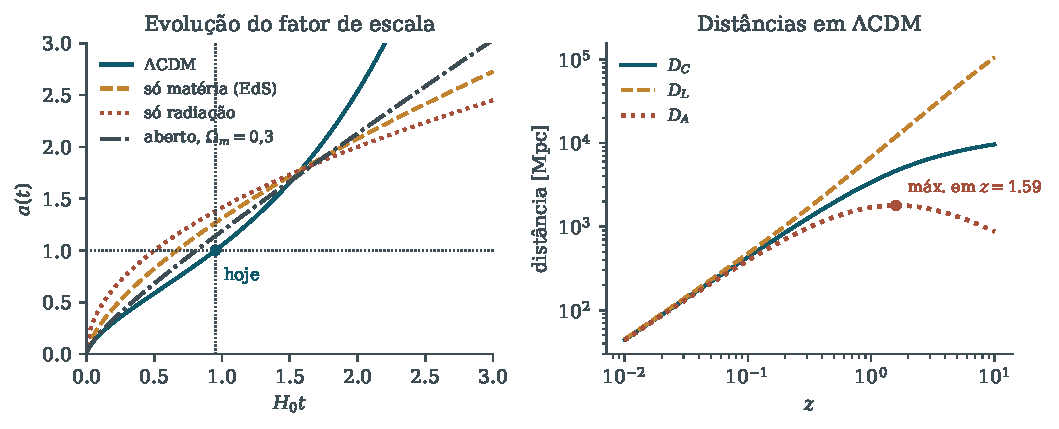
\includegraphics[width=\linewidth]{figuras/cap12_friedmann.pdf}
  \caption{À esquerda, $a(t)$ para quatro universos. Todos passam pela mesma
  origem, mas $\Lambda$CDM é o único que muda de concavidade: a curva
  desacelera enquanto a matéria domina e volta a acelerar depois. O universo
  aberto expande para sempre sem nunca acelerar. À direita, as três
  distâncias: $D_{L}$ cresce sem limite, mas $D_{A}$ tem um máximo em
  $z \approx 1{,}59$ --- objetos mais distantes que isso aparecem
  \emph{maiores} no céu.}
  \label{fig:cap13-friedmann}
\end{figure}

\subsubsection*{Distâncias e horizontes}

\begin{saida}
\begin{lstlisting}[style=rgsaida]
     z    D_C [Mpc]    D_L [Mpc]    D_A [Mpc]
   0.1        434.1        477.5        394.6
   0.5       1951.3       2927.0       1300.9
   1.0       3401.0       6802.1       1700.5
   2.0       5311.3      15934.0       1770.4
   5.0       7943.8      47662.6       1324.0
1100.0      13866.3   15266789.6         12.6

maximo de D_A em z = 1.5877, D_A = 1794.1 Mpc
horizonte de particulas hoje = 14144.3 Mpc = 46.13 Glyr
\end{lstlisting}
\end{saida}

\begin{atencao}
A última linha da tabela é a que mais confunde. Na superfície de último
espalhamento, $z \approx 1100$, a distância de diâmetro angular vale
$13$~Mpc: a mesma superfície cuja distância comóvel é de $13{,}9$~Gpc. Não há
contradição --- são grandezas diferentes, ligadas por
$D_{A} = D_{C}/(1+z)$, e é $D_{A}$ que converte tamanho físico em ângulo
observado. É por isso que o horizonte acústico da CMB, de cerca de
$150$~Mpc comóveis, subtende aproximadamente um grau no céu. Trocar $D_{A}$
por $D_{C}$ nessa conta erra o resultado por um fator de mil.

Note ainda que o horizonte de partículas, $46$~Glyr, é maior que $c t_{0}
= 13{,}8$~Glyr. Isso não viola nada: a luz percorreu $13{,}8$~Gyr de
\emph{tempo}, mas o espaço por onde ela passou continuou se expandindo.
\end{atencao}

\subsection{Mathematica}

\programa[Derivação das equações de Friedmann a partir da métrica FLRW e a solução fechada em $\sinh^{2/3}$.]{codigo/cap12\_friedmann\_simbolico.wl}

O bloco simbólico faz aqui o que o numérico não pode fazer: deriva as
equações de Friedmann a partir da métrica, em vez de assumi-las. É o mesmo
maquinário do Capítulo~\ref{cap:einstein}, aplicado à métrica de
Robertson--Walker.

A componente $rr$, combinada com a anterior, devolve
$\ddot a/a = -(4\pi/3)(\rho + 3p)$, e a divergência covariante de $T^{\mu\nu}$
devolve $\dot\rho + 3H(\rho + p) = 0$.

\begin{central}
A equação de continuidade \emph{não} é uma terceira equação independente.
Ela sai das duas primeiras por causa da identidade de Bianchi contraída,
$\nabla_{\mu}G^{\mu\nu} = 0$, provada no Capítulo~\ref{cap:curvatura}. Vale
verificar isso explicitamente no notebook: é a demonstração mais concreta de
que a conservação local da matéria está costurada na geometria, e não
imposta por fora.
\end{central}

Por fim, a solução fechada para o caso plano com matéria e $\Lambda$, que
serviu de referência para o teste numérico:
\begin{equation}
  a(t) = \left(\frac{\Omega_{m}}{\Omega_{\Lambda}}\right)^{1/3}
         \sinh^{2/3}\!\left(\frac{3}{2}\sqrt{\Omega_{\Lambda}}\,H_{0}t\right),
  \qquad
  t_{0} = \frac{2}{3H_{0}\sqrt{\Omega_{\Lambda}}}
          \operatorname{arcsinh}\sqrt{\frac{\Omega_{\Lambda}}{\Omega_{m}}}.
  \label{eq:cap13-sinh}
\end{equation}

Vale contemplar essa expressão por um instante. O $\sinh^{2/3}$ contém as
duas eras: para argumento pequeno, $\sinh x \approx x$ e recuperamos
$a \propto t^{2/3}$ de Einstein--de Sitter; para argumento grande,
$\sinh x \approx e^{x}/2$ e a expansão vira exponencial. A transição entre
matéria e energia escura, que na figura aparece como uma inflexão discreta,
está inteira nessa única função.

